%~~~~~~~~ Chapter ~~~~~~~~
\chapter{Introduction}

%
% Quantum mechanics --> technological advances --> limits --> quantum control
% --> possibilities -->
%

Condensed Matter Physics is an immensely broad topic. It encompasses many different materials at different scales and with many different approaches.
This thesis sits on the theoretical side and is essentially computational, nonetheless it has the flavor of Applied Physics or even Material Science. Naturally many other paths could have been followed, experiments pursued, theoretical models deepened and many topics could be further studied, but the line has to be drawn at some point.

Through out the whole thesis the driving force has been sometimes the possibility of interesting results, regardless their ``immediate'' utility, and some times the possibility of real world application in the near/mid future.
This position, midway between applications and fundamental research, might be a bit uncomfortable since experimentalists or industry-oriented people might find it a bit vague or hypothetical whereas fundamental researchers might think of it as too narrow, or even missing the big picture.

In contrast I think this ``equidistance'' provides a privileged position to explore a number of interesting topics without loosing touch with experimental reality.
\bigskip

This whole thesis revolves around graphene and graphene-based systems. One can find a number of reasons for this: its a relatively new material, it has many physically interesting properties and the potential for plenty of applications, it draws a lot of attention form the research community...
One could say that the scientific community may have gone through an ``interest'' bubble involving graphene and, as a consequence, graphene has been advertised as a miraculous material, with the potential to change the world as we know it. This statement may be seen in \fref{topics}, where I have analyzed the book of abstract of the APS March Meeting for a number of years.
%\footnote{after 2018 the format of the pdf file changed and I did not update the parser, but anyone interested and willing is welcome to contribute}
It counts the number of abstracts containing a given term and normalizes the count to the total number of abstracts that year. This is a very rough estimate, of course, but the resulting counting is arguably related to the interest of the condensed matter community on a certain topic.

%~~~~~~~~~~~~~~~~~~~~~~~~~~ FIGURE ~~~~~~~~~~~~~~~~~~~~~~~~~%
\begin{figure}[h!]
\centering
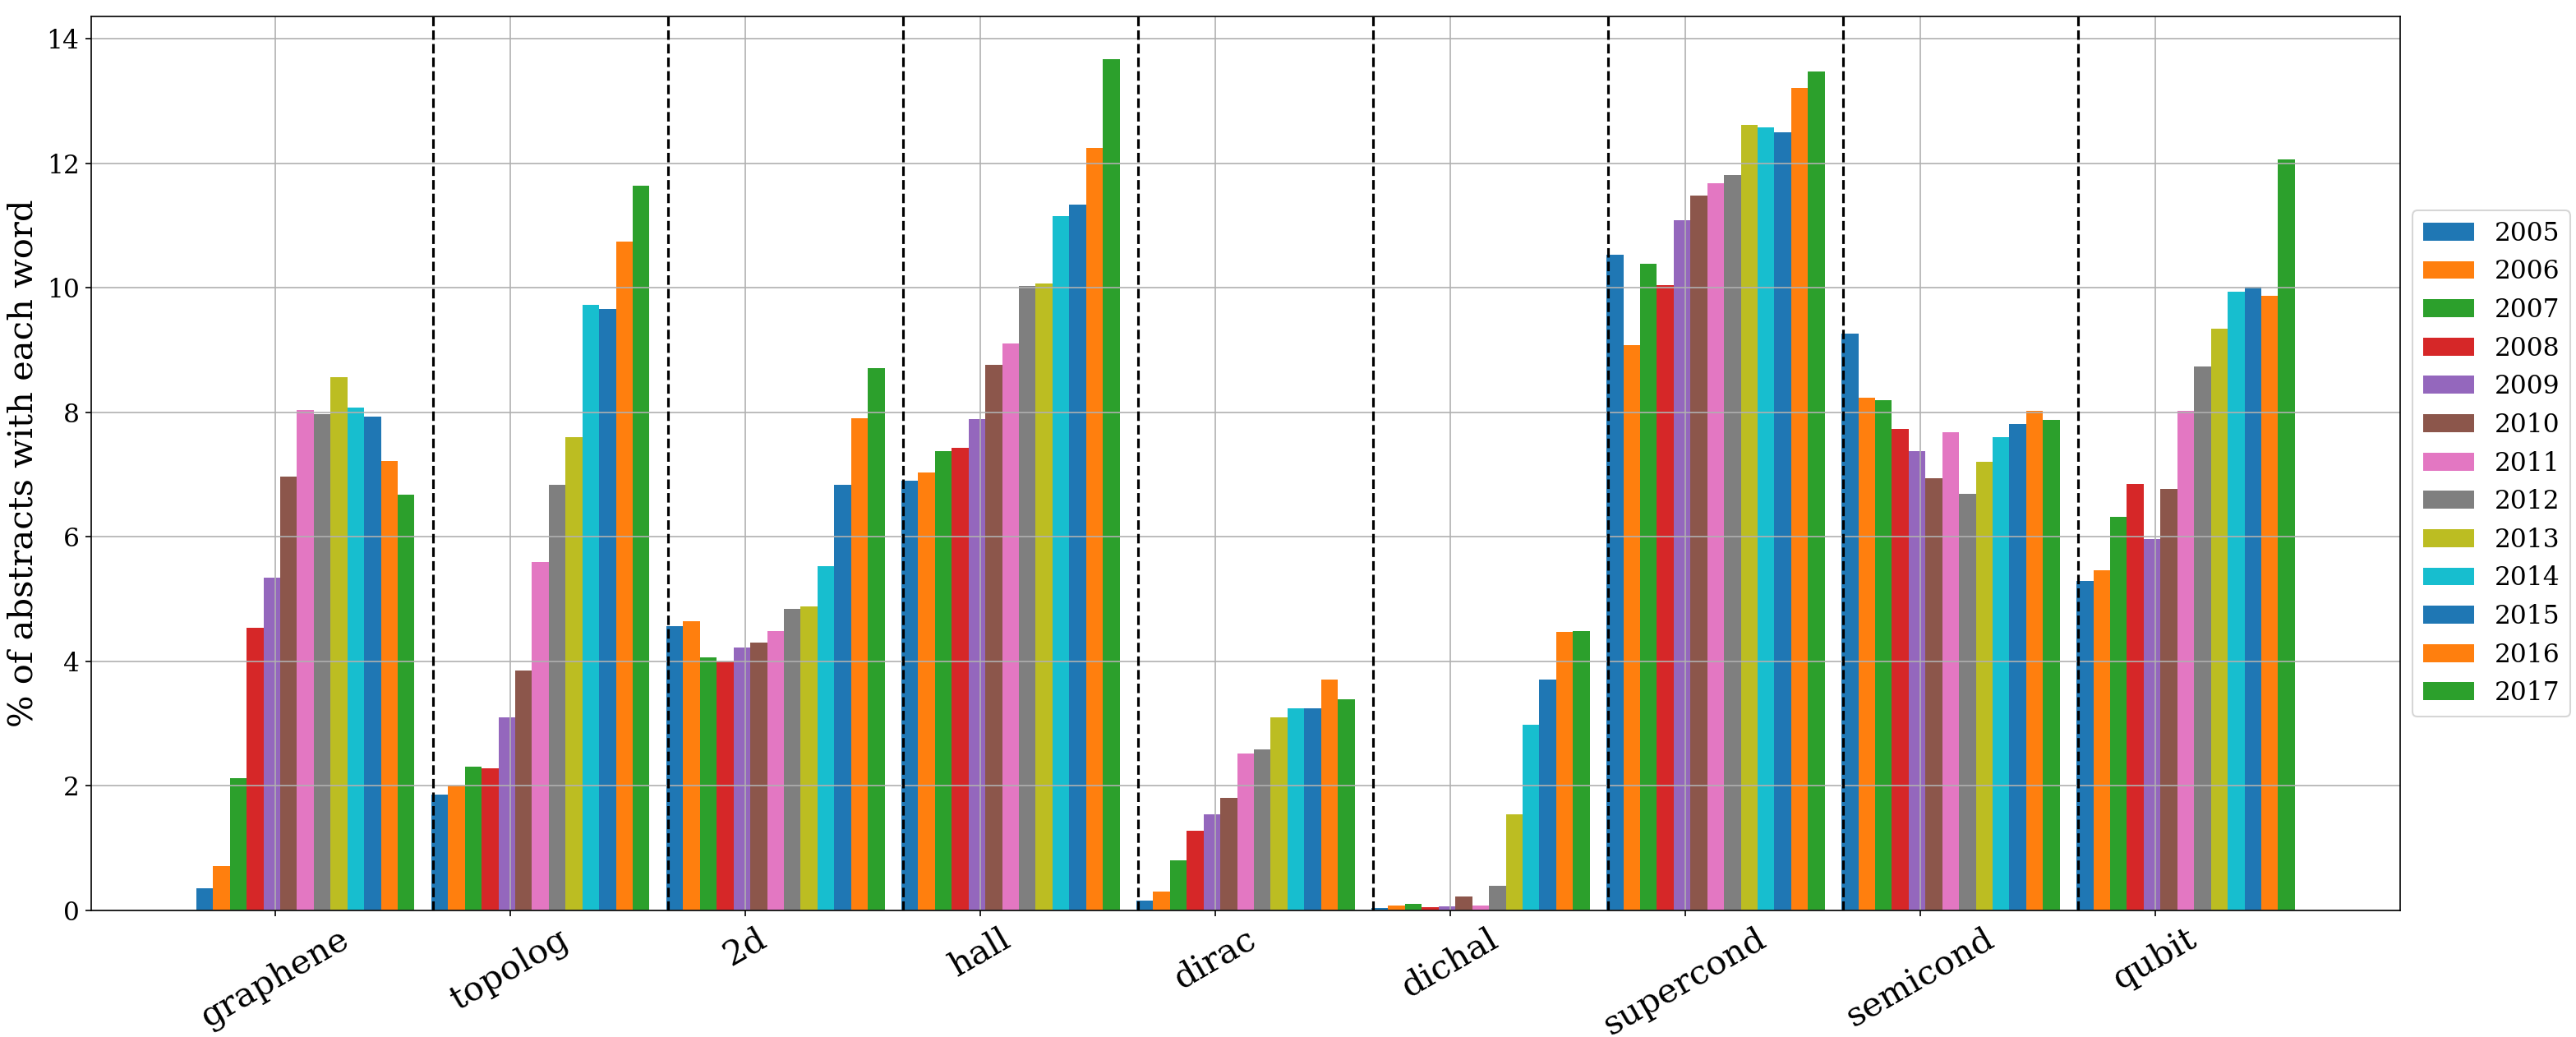
\includegraphics{introduction/figures/topics.png}
\vspace{-25pt}
\caption{Evolution through out the years of different topics at the APS March Meeting. The plot was done by counting the number of abstracts containing a given word and normalizing it by the total number of abstracts in the conference.}
\label{topics}
\end{figure}
%\FloatBarrier
%~~~~~~~~~~~~~~~~~~~~~~~~~~~~~~~~~~~~~~~~~~~~~~~~~~~~~~~~~~~%

The case of graphene is very interesting, since one can see its raise since (almost) its discovery and the beginning of its decay.

While the graphene bubble might be a real effect, I would like to point out the trend over the years of the terms next to it in \fref{topics}: topolog\textcolor{gray}{[y,ical]}, 2d, dirac, \textcolor{gray}{quantum-,spin-,anomalous-}hall, dichal\textcolor{gray}{cogenides, $MoS_2$,$WS_2$,$WSe_2$}. All of these terms are undoubtedly related to graphene an clearly they show a monotonically growing trend.
\medskip

Graphene itself is very interesting and it probably deserves all the fame and attention that it gets, but for me the importance of graphene lies in the fact that it has become the gateway for many other materials and research branches.

The understanding of graphene has been the spark to start a race in two dimensional materials research. \ac{2dm} are a very interesting family of materials both form an applied point of view and from the perspective of fundamental research.
On one hand, any industry-related property (conductance tunability, magnetism...) becomes instantly interesting just because its 2D nature ensures smaller sizes and cheaper products.
On the other hand their 2D nature place them right in the frontier between the classical and quantum regime: they are macroscopic (sometimes reaching millimeters) but being one atom thick there are non negligible quantum effects what makes the fascinating from the fundamental physics point of view.
Since its discovery many other bidimensional materials have been synthesized: Bismuth, $MoS_2$, $WeS_2$, $WSe_2$, $BN$, $CrI_3$... each with their unique set of properties and its list of possible applications.

Some of these materials will be mentioned during the thesis, but graphene will be the common thread through out the thesis.
\bigskip

One of the most interesting properties of graphene is that, being two dimensional, all of it is a surface, and electrons living in surfaces respond strongly to external perturbations.
If a superconductor is placed nearby, electrons in graphene will behave in a superconductor way\cite{},
if placed on top of an insulator it will open a gap\cite{}, if subjected to an external field its electronic states will be heavily modified.
A material in which so many different states may appear is interesting in itself, so it is no wonder why having such a panoply of different phases at their disposal, scientists quickly thought of the possibility of mixing different 2D materials in order to engineer properties at will\cite{Geim2013}.

In the spirit of these combined structures, commonly known as Van der Waals heterostructures, this thesis extensively explores the properties and applications of a bilayer of graphene.
%TODO meh....change
\bigskip

Even though it will not be discussed in the thesis, it is mandatory to comment on the recent discovery of superconductivity on bilayer graphene\cite{}
In this case the two layers need to be rotated an exact angle, what makes a moire pattern emerge. In the edges of this pattern the electrons get localized resulting on the emergence of a bunch of almost flat bands. The electron-electron interaction then, with the correct filling conspire to result in a superconductor state, in a way that is very similar to that of the case of cuprates.
While this phase is nothing new, its appearance in graphene, a system the chemistry of which has been very well known for a long time, may be a game changer. The low energy effective model of graphene is probably the most studied in the history of Condensed Matter Physics so one may expect that studying the complex problem of superconductivity would be easier in this case.
Well, it is probably too soon to tell but it looks like superconductivity will not give up its secrets so easily and even though the low energy Hamiltonian of graphene is very well known, its extension to the twisted bilayer is not so easy. Still this is a topic to keep an eye on since it may result in amazing new physics and long-waited technological applications.
\bigskip

Bilayer graphene does not fall short from the monolayer. The main property that will be exploited during the thesis is the fact that bilayer graphene undergoes a transition from conductor to insulator in the presence of an electric field.
Opening and closing a gap is a very powerful resource when dealing with electronic states since it affects the spatial localization of the electrons and many properties depend on this. In particular it is very interesting to consider a number of quasi-localized electronic states placed at the correct distance for the change in localization via gap-opening to influence their interactions.
Even, going one step further, it is not far-fetched to think of an scenario in which we can combine the this tunable gap with some spin interactions being able to tune the electronic states for each spin channel independently.
\bigskip


\newpage
This thesis has somewhat been driven, at least in part, by a proposal dating all the way back to 1988\cite{Kane1988} on how to build a \emph{quantum computer}. In this proposal Bruce E. Kane suggested Phosphorus impurities in Silicon ($Si: \leftidx{^{31}}P$) as the building block for a silicon based nuclear spin quantum computer.
Any proposal for building quantum computers (or qubits, for that matter) has to deal with the conflict between two opposing requirements. On one hand we need the qubits to be well isolated from the environment so interactions with the outside world does not affect the quantum state of the computer. On the other hand, we need to be able to interact strongly and quickly with the qubits in order to change or read its state.

The idea to tackle this contradiction was to use the nuclear spin (1/2) of the $\leftidx{^{31}}P$ to store information, due to the relatively low concentration of nuclear spins in the system, and the electric cloud around them as mediators among $P$ impurities.
The way to control the interactions would be based on the application of electric gates which would distort the electronic states increasing or decreasing the hyperfine interaction (coupling between the nuclear and the electronic spin) as well as tuning the electronic configuration in between defects.
\medbreak

Ignoring the specific nature of the materials, the relevant ingredients in this proposal are a nuclear spin 1/2, which is expected to be isolated from the rest of the universe upon the application of an electric field, An electronic spin 1/2 located somewhat around the nuclear spin and with a big response to an electric field so the interaction between the two spins can be highly tuned.



%%%%%%%%%%%%%%%%%%%%%%%%%%%%%%%%%%%%%%%%%%%%%%%%%%%%%%%%%%
\newpage

We are today on the verge of a technological revolution, a quantum leap\footnote{pun intended} that holds the promise for a revolution in chemistry, pharmacology, telecommunications, virtually any application in which optimization is a problem and even Condensed Matter Physics itself.
But let us start from the beginning.
\medbreak

The laws of \ac{qm} started developing at the beginning of the XX century. At that moment, it was commonly thought that only a few details in the laws of Physics remained unexplained, but as Physicists delved deeper in these unexplained phenomena (namely the photo-electric effect and the black body radiation), it became clear that there was some missing piece.

Step by step it was found that as the energy scales of the experiments grew smaller, the well-founded laws of \emph{classical} physics started failing.
% infrared catastrophe
% atomic model (electron radiation)
The development and understanding of the laws of \ac{qm} was fast and in merely 30 years there were entire research fields centered already in different aspects or applications of it.

Of particular interest to this thesis is the line of material science and condensed matter physics research. Prior to the understanding of \ac{qm}, there was no theory to explain the properties of any material.
Whether a piece of rock was able to conduct heat or electricity was essentially a matter of trial and error. Of course some experimental observations led Chemists to build a collection of somewhat empirical laws and group elements based on similar properties, but there was no microscopic understanding of the mechanisms leading to these properties.

The capabilities of \ac{qm} to predict electronic properties of different materials led to a revolution in science, technology and ultimately society. The extensive research on semiconductor materials during the 1960s was key to the invention of the transistor: a device that can block or allow the flow of electrical current at will.

The transistor is the basic building block for any electronic device. Nowadays there are millions if not billions of transistors in our computers or smartphones, but only a few thousand were enough to send 3 humans to the moon (and back!). For the last 50 years, transistors have operated based on the fine-tune of the band population of two neighboring materials creating an effective potential barrier between them preventing electrons to move freely.
As the electronic industry developed the need for smaller transistors became apparent, the smaller the transistors are, the more can be fit in a particular device.
This race towards miniaturization pushed the development of new materials and techniques to size down transistors all the way to the current\footnote{In mass production, there are plenty of claims for smaller transistors.} $\sim\SI{14}{\nm}$. As expected, when we shrink the components of the transistors, we approach a limit in which quantum effects irrelevant until now may take a major role. The simplest obstacle that the shrinking of transistors have to deal with is the quantum tunnel effect, by which the electrons would be able to flow through the potential barrier, rendering the transistor unable to effectively stop electric current.

Quantum effects will play an important role as technology shrinks, but this may not be necessarily a problem.


\medbreak

Quantum limit is a feature. Feynman "control of atomic properties"

Quantum computers

Quantum simulations






%%%%%%%%%%%%%%%%%%%%%%%%%%%%%%%%%%%%%%%%%%%%%%%%%%%%%%%%%%%%%%%%%%%%%%%%%%%%%%%%
\newpage
The development of Quantum Technologies has barely started and it already promises a revolution in many different fields, from medicine and pharmacology, computation, encryption, any application in which optimization is a problem and even the understanding of quantum mechanics itself.
There is probably nothing riskier than trying to make technological predictions, but even governments around the world are taking action to be in the forefront of this revolution\cite{QTF} and big companies such as Google, IBM or Microsoft are investing huge amounts of money in these topics. But let us start from the beginning.
\medbreak

% Quantum technologies
Nowadays we are barely getting a glimpse of the potential of quantum technologies to impact technology and science in general, but Quantum computation is not something that we just thought about.
Ever since we started the race to shrink every computer component, we headed towards the limit of quantum computation. A transistor is a device able to switch on and off an electrical current on command. They are the basic building block for any kind of computerized device. The first transistors were macroscopic, some centimeters and wired by hand. As the potential of computers grew, the need to create more, cheaper and smaller transistors launched the race for miniaturization. %Moore's Law is the empir
Nowadays a single transistor is the size of a few nanometers. At this scale  quantum effects start playing a significant role.
If there is a potential barrier stopping the electric current and it becomes smaller and smaller at some point the tunnel effect will be probable enough to render the transistor unable to stop any electric current at all.
This is one of the simplest limitations that computers face as we miniaturize components.

While it may seem that dealing with the inevitable quantum effects is a big inconvenience, scientists began to consider the possibility of using these effects to our benefit.
The first ideas about the possibilities for quantum computing started in the 80s and 90s\cite{Benioff1980, Feynman1982, Manin1980, Shor1994} showed that a quantum computer could tackle problems that a classical computer simply could not.

Since then there has been huge developments both theoretical and experimental towards the realization of a platform in which to perform \emph{quantum computations}.




\medbreak


% Graphene
In general, states near surfaces are very susceptible to external biases. In particular, \ac{2d} materials present highly manipulable electronic states since they only have the surface to live in.
Even before its discovery, graphene has drawn a lot of attention. Many of its properties were expected well twenty years before its experimental discovery. While it is arguably true that there has been an over-hype bubble around its supposed miraculous applications, it is definitely true that graphene has been the gateway towards a whole new realm of phenomena in condensed matter physics. 

Initially most of its interest relied in the expectancy of a new Hall phase emerging without the need of an external magnetic field\cite{Kane2005a,Ostrovsky2008} and the experimental observation of the \ac{qhe}, a macroscopic effect of a purely quantum phenomenon\cite{Zhang2005}.
Also fact that some high-energy physics models were naturally realized in graphene was a huge motivation for this material to hoard the attention of a big part of the condensed matter community.

Certainly graphene has many interesting properties, but when two layers of graphene are placed one on top of each other there is a property that will be central for the development of this thesis.

Graphene bilayer is the only known material which can open a gap upon application of an electric field. It has been shown that an electric




%\newpage
%In order to start wrapping our minds around this Quantum Revolution, we need to look back to the beginning of the XIX century. Back then Physics was consider to be completely understood, except for a couple of seemingly simple experiments, namely the photoelectric effect and the black body radiation. These phenomena were the gateway to discover the realm of Quantum Mechanics.
%
%Many experiments followed and the theory was not left behind. Soon we had a framework with the mathematical tools to describe all these new phenomena. Nevertheless having the basic laws that rule this 
%
%
%\medbreak
%The world has seen all sorts of revolutions all throughout history. While not necessarily every revolution has turned the world into a better place, when we account just for the scientific or technological revolutions, this is usually the case.
%
%%At the end of the XVIII century, the invention of the steam engine and its later introduction in the industrial processes allowed a huge step forward for many societies and, for better or worse\cite{}%climate
%%, reshaped the world.
%%The Industrial Revolution changed the way we travel and work, it changed the scale at which humans interacted with the planet and, arguably, the universe.
%%The whole world has seen how virtually any index measuring quality of life has been raising ever since\cite{}.\footnote{Sadly this trend has not been homogeneous at all around the globe and these changes have been much more clear in some countries than others.}
%
%%Similarly, another huge revolution came along with
%The worldwide introduction of computers in most households and the construction of a worldwide web interconnecting ``everyone'' in the world has been one of the biggest revolutions over the last 30 years. The information technologies have changed the job-market landscape, the way humans learn, shop, the way we socialize even the way we fight wars. Even in their first stages computers were able to put two men on the moon and bring them back with less computational power than the cheapest smartphone available today.
%Our daily habits, our leisure time, even crucial historical events\cite{Alhindi2012} have been determined by the use of computers and the internet.
%
%For this revolution to happen, many agents had to be in place. The need for secure communication channels during World War II pushed the development of information theory and the later Cold War pushed scientists and engineers to build computers. But the bare necessity is not enough to develop the necessary technology. The first computers used \emph{macroscopic transistors} and \emph{macroscopic bits} when they were introduced. At first these essential pieces were handmade and manufactured one by one. It was not until the research in semiconductor physics developed microscopic versions of these pieces that the computers became cheap and easy to produce.
%\medbreak
%
%\newpage
%For nowadays computers to exist, it was necessary the development of Quantum Mechanics. Starting with the beginning of the XX century, physicist realised that Physics was not completely understood but rather there were many mysteries when 
%
%
%
%Naturally these revolutions did not just happen, it took many years of hard work and research to stablish the basis for these technologies to emerge. In particular, for computers to be created and be popularized it was necessary a deep understanding of the laws of quantum physics which led to the mastery of the semiconductor technologies.
%
%
%
%\newpage
%
%%%%%%%%%%%%%%%%%%%%%%%%%%%%%%%%%%%%%%%%%%%%%%%%%%%%%%%%%%%%%%%%%%%%%%%%%%%%%%%%%
%The relation between research in fundamental Physics and technological innovations is not always easy to see. In the best of cases, it usually takes some years, at least a few decades, for fundamental research to find its way into the industry.
%While this is a completely fair question, it is quite short-sighted. Let us think of the latest revolution that changed our society.
%The introduction of computers in our everyday life and the access to a global network of communications was a revolution, maybe even comparable to the industrial revolution.
%
%We have had computers in most households for the last 30 years, broad access to the internet for over 20, yet, trying to pin-point the fundamental research that took us there is quite hard, if not impossible.
%We can think of the first transistor\footnote{actually there is a previous patent, from 1930,\cite{diode} but no hard proof that it was ever built or used.},
%the building block of every electronic device, which would take us to the 40's\cite{Ross}, but it would be unimaginable to reach that point without at least some understanding of the physics of semiconductors which had been studied for the previous 50 years. It would be insane trying to understand semiconductors without, at least, a few notions of quantum mechanics, electromagnetism...
%We could line up all the most brilliant minds of humanity that set the path towards today's technology: Landau, Bardeen, Bloch Dirac, Heisenberg, Bragg, Brillouin, Faraday, Gauss... countless others... Ask them about the application of their research, and not one of them would be able to describe a personal computer or the internet.
%
%That is why asking the researchers about the usefulness of their research is like asking newborn babies what will be their job position in 42 years time.
%
%Of course we have our own vision of what the research may bring upon the world, but let us keep in mind that this vision is nothing but a childish dream, since time and time again the applications have exceeded the wildest expectations of the researchers.\\
%
%
%At the end of the XIX century it was believed that Physics was solved. Today we know it is not. In particular, Condensed Matter Physics is an area in which even when we know the physical laws governing every interaction there is still much that we do not understand. Quantum Mechanics gives us the tools to describe any problem that we want to describe. From superconductors to topological phases or spin liquids, the Hamiltonian is known and yet we cannot solve it. The last fifty or sixty years of condensed matter physicist have been devoted to approximations and simplifications that would allow us to strip the problems to its basic components in an attempt to understand the microscopical mechanism behind so many interesting phenomena.
%The thorough investigation of a variety of problems while not completely successful in every area, has had a great side effect. The cumulative experience of decades of condensed matter physics research has granted us the ability to control matter with atomic precision in a wide range of situations. The fulfillment of such a dream\cite{Feynman1982}
%
%Quantum technologies\cite{QTF}
%
%The research on semiconductor physics can be hard to pin-point, 
%
%
%In this work we study a variety of properties regarding defected graphene bilayer. Starting from the basic concepts of graphene, we build our way to the role of sp$^3$-defects in graphene bilayer such as chemisorbed Hydrogen adatoms.
%First we study the properties of these defects one by one in isolated scenarios. Then we wonder the effects of neighboring defects
